%%%%%%%%%%%%%%%%%%%%%%%%%%%%%%%%%%%%%%%%%
% Beamer Presentation
% LaTeX Template
% Version 1.0 (10/11/12)
%
% This template has been downloaded from:
% http://www.LaTeXTemplates.com
%
% License:
% CC BY-NC-SA 3.0 (http://creativecommons.org/licenses/by-nc-sa/3.0/)
%
%%%%%%%%%%%%%%%%%%%%%%%%%%%%%%%%%%%%%%%%%

%----------------------------------------------------------------------------------------
%	PACKAGES AND THEMES
%----------------------------------------------------------------------------------------

\documentclass{beamer}

\mode<presentation> {

% The Beamer class comes with a number of default slide themes
% which change the colors and layouts of slides. Below this is a list
% of all the themes, uncomment each in turn to see what they look like.

%\usetheme{default}
%\usetheme{AnnArbor}
%\usetheme{Antibes}
%\usetheme{Bergen}
%\usetheme{Berkeley}
%\usetheme{Berlin}
%\usetheme{Boadilla}
%\usetheme{CambridgeUS}
%\usetheme{Copenhagen}
\usetheme{Darmstadt}
%\usetheme{Dresden}
%\usetheme{Frankfurt}
%\usetheme{Goettingen}
%\usetheme{Hannover}
%\usetheme{Ilmenau}
%\usetheme{JuanLesPins}
%\usetheme{Luebeck}
%\usetheme{Madrid}
%*\usetheme{Malmoe}
%\usetheme{Marburg}
%\usetheme{Montpellier}
%\usetheme{PaloAlto}
%\usetheme{Pittsburgh}
%\usetheme{Rochester}
%\usetheme{Singapore}
%\usetheme{Szeged}
%\usetheme{Warsaw}

% As well as themes, the Beamer class has a number of color themes
% for any slide theme. Uncomment each of these in turn to see how it
% changes the colors of your current slide theme.

%\usecolortheme{albatross}
%\usecolortheme{beaver}
%\usecolortheme{beetle}
%\usecolortheme{crane}
%\usecolortheme{dolphin}
%\usecolortheme{dove}
%\usecolortheme{fly}
%\usecolortheme{lily}
\usecolortheme{orchid}
%\usecolortheme{rose}
%\usecolortheme{seagull}
%\usecolortheme{seahorse}
%\usecolortheme{whale}
%\usecolortheme{wolverine}

%\setbeamertemplate{footline} % To remove the footer line in all slides uncomment this line
%\setbeamertemplate{footline}[page number] % To replace the footer line in all slides with a simple slide count uncomment this line

%\setbeamertemplate{navigation symbols}{} % To remove the navigation symbols from the bottom of all slides uncomment this line
}


\usepackage{graphicx} % Allows including images
\usepackage{booktabs} % Allows the use of \toprule, \midrule and \bottomrule in tables
\usepackage{xspace}
\usepackage{caption}
\usepackage{subfigure}
\usepackage[english,brazil]{babel}
\usepackage[utf8]{inputenc}

%Renomeia o nome padrao das figuras.
\renewcommand{\figurename}{Figura}
\renewcommand{\tablename}{Tabela}
%----------------------------------------------------------------------------------------
%	TITLE PAGE
%----------------------------------------------------------------------------------------

\title[Computação Gráfica]{Modelo de Iluminação} % The short title appears at the bottom of every slide, the full title is only on the title page

\author{Uéliton Freitas} % Your name
\institute[UFMS] % Your institution as it will appear on the bottom of every slide, may be shorthand to save space
{
Universidade Católica Don Bosco - UCDB \\ % Your institution for the title page
\medskip
\textit{freitas.ueliton@gmail.com} % Your email address
}
\date{\today} % Date, can be changed to a custom date


\begin{document}

\begin{frame}
\titlepage % Print the title page as the first slide
\end{frame}

\begin{frame}
\frametitle{Sumário} % Table of contents slide, comment this block out to remove it
\tableofcontents % Throughout your presentation, if you choose to use \section{} and \subsection{} commands, these will automatically be printed on this slide as an overview of your presentation
\end{frame}




%----------------------------------------------------------------------------------------
%	PRESENTATION SLIDES
%----------------------------------------------------------------------------------------

%------------------------------------------------
\section{Introdução} 
%------------------------------------------------

%\section{Speeded-Up Robust Features - SURF} % A subsection can be created just before a set of slides with a common theme to further break down your presentation into chunks
%\section{Baf Of Features and Colors}

%\section{Refer\^encias}
%%%%%%%%%%%%%%%%%%%%%%%%%%%%%%%%%%%%%%%%%%%%%%%%%%%%%%%%%%%%%%%%%%%%%%%%%%%%%%%%%%%%%%%%%%
\begin{frame}
\frametitle{Introdução}

		\begin{block}{Introdução}
		\begin{itemize}
			\item Os modelos físicos envolvem vários fatores como \textbf{propriedade dos materiais},\textbf{posições} dos objetos em relação a luz e outros objetos, além das características das fontes de luz.
			\begin{itemize}
				\item Os objetos podem ser transparentes ou opacos, podem ser finos ou  mais grosseiros.
				\item Fontes de luz podem ter vários formatos, cores e posições.
			\end{itemize}
			\item Os \textbf{Modelos de Iluminação} em computação gráfica são, na maioria das vezes, \textbf{aproximações} das leis da física que descrevem efeitos de luz sobre as superfícies.			 
		\end{itemize}
	\end{block}
	
\end{frame}



%%%%%%%%%%%%%%%%%%%%%%%%%%%%%%%%%%%%%%%%%%%%%%%%%%%%%%%%%%%%%%%%%%%%%%%%%%%%%%%%%%%%%%%%%%
\section{Fontes de Luz}
\begin{frame}
\frametitle{Fontes de Luz}

	\begin{block}{Fontes de Luz}
		\begin{itemize}
			\item Qualquer objeto brilhante é uma \textbf{fonte de luz} e emite luz e contribui para os efeitos de luz dos outros objetos da cena.
			\item \textbf{Fontes de Luz} podem ter diferentes formas e características (posição, cor, direção de emissão) podendo emitir ou refletir luz.
			\item Em aplicações gráficas de \textbf{tempo real}, muitas vezes são utilizados modelos simples de iluminação para obter um melhor \textbf{custo computacional}.
		\end{itemize}
	\end{block}
\end{frame}

%%%%%%%%%%%%%%%%%%%%%%%%%%%%%%%%%%%%%%%%%%%%%%%%%%%%%%%%%%%%%%%%%%%%%%%%%%%%%%%%%%%%%%%%%%
\begin{frame}
\frametitle{Fontes de Luz}

	\begin{block}{Fonte de Luz Puntual}
		\begin{itemize}
			\item É o modelo de luz mais simples.
			\begin{itemize}
				\item Possui uma posição.
				\item Defini-se a cor que será emitida.
				\item Os raios de luz são gerados em \textbf{direções radiais divergentes} a partir do ponto da luz.
			\end{itemize}
		\end{itemize}
	\end{block}
		\begin{figure}[!h]
			\begin{center}
			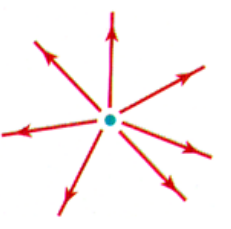
\includegraphics[width=0.2\textwidth]{Figures/FonPun}
			\end{center}
		\end{figure}
\end{frame}

%%%%%%%%%%%%%%%%%%%%%%%%%%%%%%%%%%%%%%%%%%%%%%%%%%%%%%%%%%%%%%%%%%%%%%%%%%%%%%%%%%%%%%%%%%
\begin{frame}
\frametitle{Fontes de Luz}

	\begin{block}{Fonte de Luz Infinitamente Distantes}
		\begin{itemize}
			\item Uma fonte de luz grande(p.ex Sol) que está bem longe da cena pode ser aproximado com um ponto emissor bem distante dos objetos.
			\begin{itemize}
				\item A iluminação é provida em uma única direção.
			\end{itemize}
			\item Uma fonte de luz distante é simulada definindo uma \textbf{cor} e uma \textbf{direção} de emissão de raios. Não é necessário definir uma posição.
		\end{itemize}
	\end{block}
		\begin{figure}[!h]
			\begin{center}
			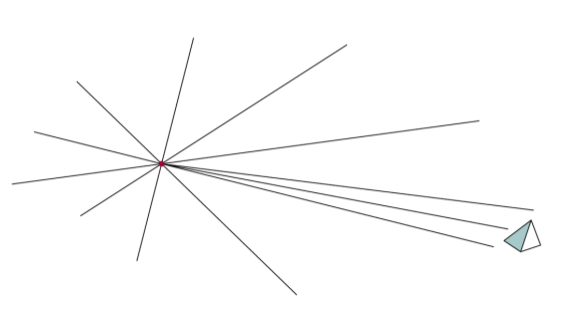
\includegraphics[width=0.6\textwidth]{Figures/FonDis}
			\end{center}
	\end{figure}
\end{frame}

%%%%%%%%%%%%%%%%%%%%%%%%%%%%%%%%%%%%%%%%%%%%%%%%%%%%%%%%%%%%%%%%%%%%%%%%%%%%%%%%%%%%%%%%%%
\begin{frame}
\frametitle{Fontes de Luz}

	\begin{block}{Atenuação Radial da Intensidade}
		\begin{itemize}
			\item A energia de radiação de uma fonte de luz em uma distância $d_l$ da origem, tem sua \textbf{amplitude} atenuada  por um fator $\frac{1}{d^{2}_{l}}$.
			\begin{itemize}
				\item Uma superfície próxima a fonte de luz recebe maior intensidade de luz.
				\item Para uma \textbf{iluminação realística} esta atenuação deve ser considerada.
			\end{itemize}
			\item Na prática uma atenuação $\frac{1}{d^{2}_{l}}$ para fontes de luz puntuais não produz efeitos realísticos.
			\begin{itemize}
				\item Há uma alta variação de intensidade em objetos próximos a fonte de luz e uma baixa variação para objetos que estão longe da fonte.
			\end{itemize}
		\end{itemize}
	\end{block}
\end{frame}

%%%%%%%%%%%%%%%%%%%%%%%%%%%%%%%%%%%%%%%%%%%%%%%%%%%%%%%%%%%%%%%%%%%%%%%%%%%%%%%%%%%%%%%%%%
\begin{frame}
\frametitle{Fontes de Luz}

	\begin{block}{Atenuação Radial da Intensidade}
		\begin{itemize}
			\item Para produzir efeitos mais realísticos com fonte de luz puntuais usamos:
				\begin{equation*}
					f(d_l) = \frac{1}{a_0 + a_1d_l + a_2d^{2}_{l}}
				\end{equation*}
			\item Os valores de $a_0,a_1$ e $a_2$ podem ser ajustados para produzir efeitos de atenuações desejados.
			\begin{itemize}
				\item Valores grandes podem ser assinalados para $a_0$ quando $d_l$ é muito pequeno para prevenir que $f(d_l)$ de ficar muito grande.
			\end{itemize}
		\end{itemize}
	\end{block}
\end{frame}

%%%%%%%%%%%%%%%%%%%%%%%%%%%%%%%%%%%%%%%%%%%%%%%%%%%%%%%%%%%%%%%%%%%%%%%%%%%%%%%%%%%%%%%%%%
\begin{frame}
\frametitle{Fontes de Luz}

	\begin{block}{Atenuação Radial da Intensidade}
		\begin{itemize}
			\item Este cálculo não pode ser aplicado para fontes de luz no ``infinito'' porque a distância $d_l$ é indeterminada.
			\item Um outro problema que é que quase todos os pontos estarão a mesma distância da fonte de luz. (baixo realismo).
			\item Para resolver o problema:
			\begin{equation*}
				f(d_l) = \Big{(
  \begin{array}{l l}
    1 & \quad \text{se a fonte de luz está no infinito}\\
    \frac{1}{a_0 + a_1d_l + a_2d^{2}_{l}} & \quad \text{se a fonte de luz é local}
  \end{array} }
			\end{equation*}			 
		\end{itemize}
	\end{block}
\end{frame}


%%%%%%%%%%%%%%%%%%%%%%%%%%%%%%%%%%%%%%%%%%%%%%%%%%%%%%%%%%%%%%%%%%%%%%%%%%%%%%%%%%%%%%%%%%
\section{Fontes de Luz Direcional e Efeito de Holofote}
\begin{frame}
\frametitle{Fontes de Luz}

	\begin{block}{Atenuação Radial da Intensidade}
		\begin{itemize}
			\item Uma fonte e luz pontual pode ser direcionada para produzir um efeito de \textbf{luz direcional} ou holofote.
			\begin{itemize}
				\item Se o objeto está fora dos limites direcionais ele é eliminado da iluminação.
			\end{itemize}
			\item Uma \textbf{fonte de luz direcional} pode ser definida por uma \textbf{posição}, um \textbf{vetor direcional} e um limite angular $\theta$ a partir deste vetor.				 
		\end{itemize}
	\end{block}

	\begin{figure}[!h]
			\begin{center}
			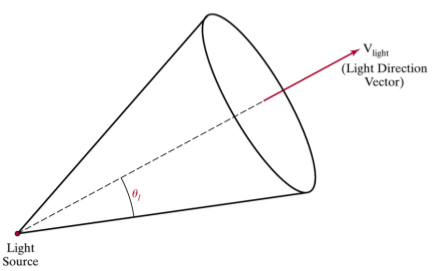
\includegraphics[width=0.48\textwidth]{Figures/Hol}
			\end{center}
	\end{figure}	
	
\end{frame}

%----------------------------------------------------------------------------------------
\end{document} 